\section{Verbale della riunione}
\subsection{Discussione data di consegna dei documenti RQ}
Dopo aver discusso brevemente le varie date possibili, abbiamo deciso di consegnare i documenti per RQ il 2021-04-27.
\subsection{Discussione ultime modifiche dei documenti}
Discussione sullo stato di avanzamento dei vari documenti.
\begin{itemize}
	\item {\textbf{Norme di Progetto:}} quasi completate;
	\item {\textbf{Piano di Qualifica:}} 
		\begin{itemize}
			\item Aggiornare sezioni sui test, aggiungendo i nuovi test di unità;
			\item Aggiornare il cruscotto web;
			\item Aggiungere le considerazioni dell'ultimo periodo;
			\item Aggiungere esito dei test di accettazione e unità nel cruscotto web;
			\item Utilizzare checkstyle per l'analisi statica lato java;
		\end{itemize} 
	\item {\textbf{Piano di Progetto:}} Aggiornare preventivi di periodo e consuntivi;
	\item {\textbf{Analisi dei Requisiti:}} Aggiungere i nuovi requisiti.
\end{itemize}
\subsection{Discussione redazione manuale manutentore}
Divisione della redazione del manuale manutentore tra i membri.
\begin{itemize}
	\item {Sezione 1:} Tessari Andrea;
	\item {Sezione 2:} De Renzis Simone, Chiarello Sofia e Greggio Nicolò;
	\item {Sezione 3:} Tessari Andrea;
	\item {Sezione 4:} Crivellari Alberto;
	\item {Sezione 5:} De Renzis Simone e Greggio Nicolò;
	\item {Sezione 6:} De Renzis Simone e Greggio Nicolò.
\end{itemize}
\pagebreak
\subsection{Contatto con il proponente via chat}
Scambio di messaggi via Google Chat con il proponente.
\begin{itemize}
	\item Domanda:
	\begin{figure}[H]
		\centering
		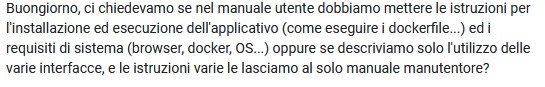
\includegraphics[scale=0.55]{res/images/screen0.jpg}
	\end{figure}	
	\item Risposta:
	\begin{figure}[H]
		\centering
		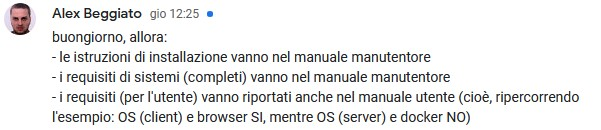
\includegraphics[scale=0.55]{res/images/screen1.jpg}
	\end{figure}		
	\item Domanda:
	\begin{figure}[H]
		\centering
		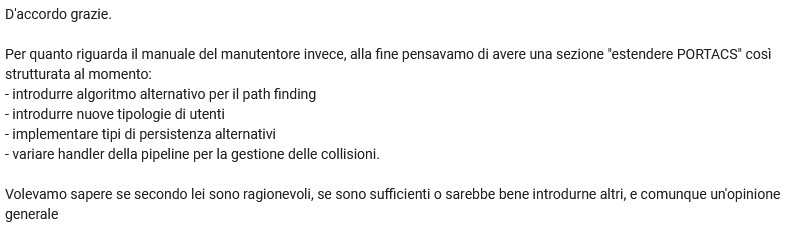
\includegraphics[scale=0.55]{res/images/screen3.jpg}
	\end{figure}
	\item Risposta:	
	\begin{figure}[H]
		\centering
		
\includegraphics[scale=0.55]{res/images/screen2.jpg}
	\end{figure}
\end{itemize}


